\documentclass[11pt]{article}
\usepackage{graphicx}
\usepackage{amsmath,amsthm,amsfonts}
\usepackage{epsfig,graphics}
\usepackage{hyperref}
\usepackage{verbatim}
\usepackage{mathrsfs}
\usepackage{fancyhdr}

\setlength{\textheight}{8.5in}
\setlength{\evensidemargin}{0.0in}
\setlength{\oddsidemargin}{0.0in}
\setlength{\topmargin}{-0.5in}
\setlength{\textwidth}{6.5in}

\newtheorem{theorem}{Theorem}
\newtheorem*{theorem*}{Theorem}
\newtheorem{claim}{Claim}
\newtheorem*{claim*}{Claim}
\newtheorem{lemma}{Lemma}
\newtheorem*{lemma*}{Lemma}
\newtheorem{exercise}{Exercise}
\newtheorem*{exercise*}{Exercise}
\newtheorem{corollary}{Corollary}
\theoremstyle{definition}
\newtheorem{definition}{Definition}
\newtheorem{fact}{Fact}
\newtheorem*{fact*}{Fact}


\pagestyle{fancy}
\fancyhf{}

%\newcommand{\lecture}[5]{\handout{#1}{#2}{#3}{#4}{#5}}


% Types of Variables
\newcommand{\bvar}[1]{\mathbf{#1}} % bold variable
\newcommand{\mvar}[1]{\bvar{#1}} % matrix variable
\newcommand{\vvar}[1]{\vec{#1}} % vector variable

% Domains
\newcommand{\R}{\mathbb{R}}
\newcommand{\Z}{\mathbb{Z}}
\newcommand{\redgevec}{\R^{E}}
\newcommand{\rvertvec}{\R^{V}}
\newcommand{\rPos}{\R^{+}}
\newcommand{\rNonNeg}{\R^{\geq 0}}

% Probability Operators
\newcommand{\E}{{\mathbb{E}}}
\newcommand{\V}{{\text{Var}}}
\newcommand{\prob}{{\mathbb{P}}}

% Symbol for definitions
\newcommand{\defeq}{\stackrel{\mathrm{\scriptscriptstyle def}}{=}}

% Optimization
\DeclareMathOperator*{\argmin}{arg\,min}
\DeclareMathOperator{\Cone}{Cone}
\DeclareMathOperator{\Cut}{CUT}

% Types of Graphs
\newcommand{\nlap}{\mathscr{L}_G}
\newcommand{\pseudo}[1]{{#1}^\dagger}
\newcommand{\lapPseudo}{\pseudo{\lap}}
\newcommand{\adj}{A}
\newcommand{\incMatrix}{\mvar{B}}
\newcommand{\diag}{\operatorname{diag}}
\newcommand{\rMatrix}{\mvar{R}} % resistance matrix
\newcommand{\iMatrix}{\mvar{I}} % identity matrix
\newcommand{\Vol}{\textrm{Vol}}


% Vectors
\newcommand{\1}{\vec{1}}
\renewcommand{\dot}[1]{\langle {#1} \rangle}

%other
\DeclareMathOperator{\sgn}{sgn}


\graphicspath{{pictures/}}


\lhead{MA 881: Lecture 9.11.18}
\rhead{Benjamin Draves}

\begin{document}

\section{Introduction } 

First, we layout the biological structure we are attempting to study. In each cell there are 23 pairs of chromosomes that include several genes. Each gene is ``expressed'' at varying levels. This expression is typically measured by something called \textit{mRNA transcripts}. mRNA sequences are a key coding to protein creation. In particular RNA codes the DNA with respect to some reference strand (usually 5'). Cells transcribe these mRNA sequences and then discard introns that have no relevant coding information for protein creation. After this step, the mRNA exits the nucleus to code the creation of proteins.
\begin{figure}[h!]
	\centering
	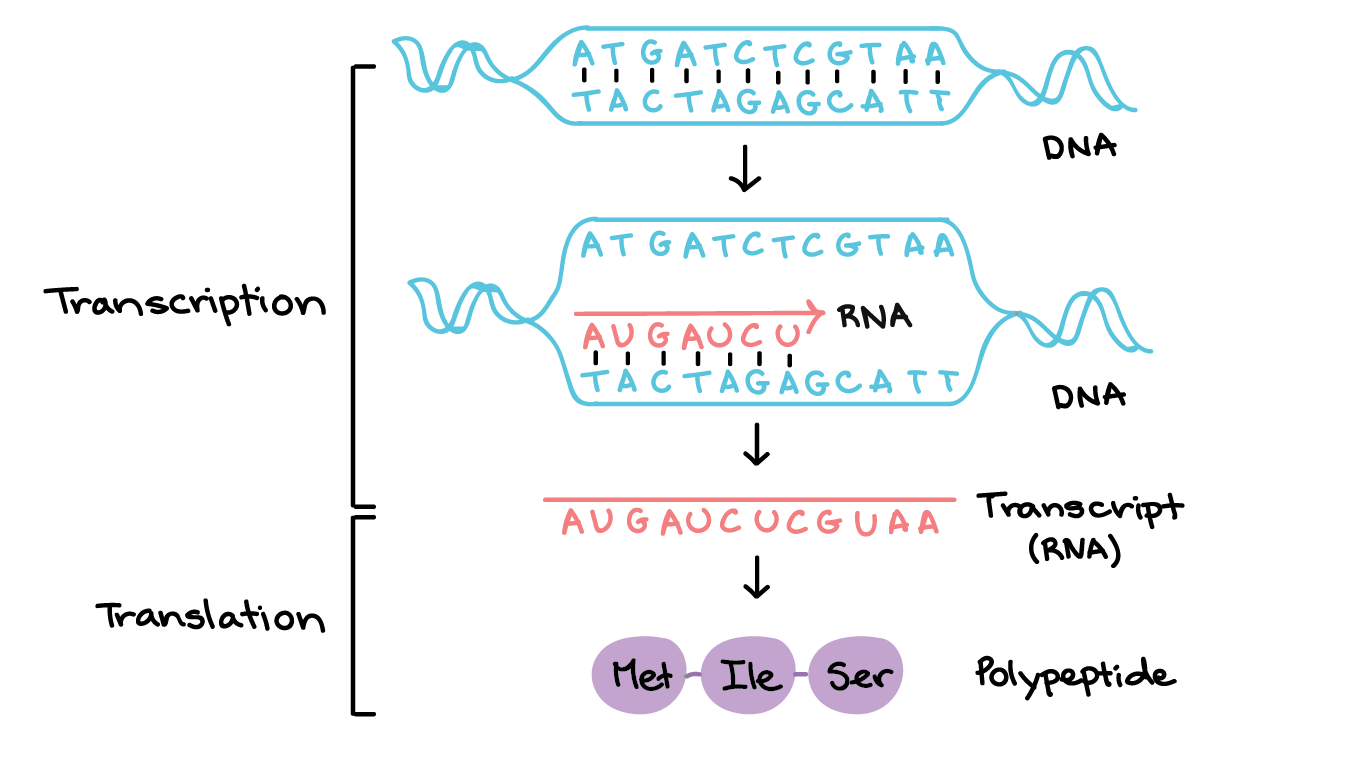
\includegraphics{transcription.png}
	\caption{A visual representation of RNA transcription.}
\end{figure}
In high-throughput analysis we wish to measure gene expression or gene activity. One way in which we can do this is to count, at some point in time, the number or mRNA transcriptions the cell is producing from each gene. The thought process being that if more proteins are being coded by gene $i$ then gene $j$ then gene $i$ is more active than gene $j$. 
\begin{figure}[h!]
	\centering
	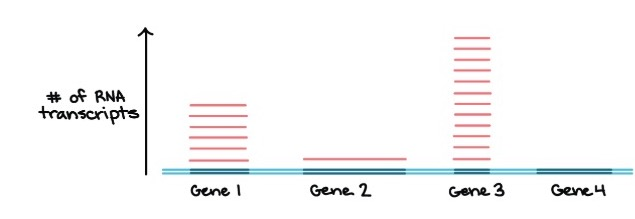
\includegraphics[scale = 0.5]{gene_expression.jpg}
	\caption{A visual representation of gene expression.}
\end{figure}
These counts will serve as the basis for our analysis procedure. In that we will focus on the following data matrix 
\begin{figure}[h!]
\centering
	\begin{tabular}{c|c|c|c|c}
		Gene ID & Sample 1 & Sample 2 & \dots & Sample N\\
		\hline
		A1BG & 24 & 30 & \dots & 17\\
		ASM & 24 & 500 & \dots & 343\\
		\vdots & \vdots & \vdots & \vdots & \vdots\\ 
		B2BM & 100 & 2 & \dots & 19
	\end{tabular}
	\caption{Counting ``reads" per gene. The main data structure of our analysis.}
\end{figure}
Having established a biological motivation to the reads per gene datastructure we now turn to actually collecting this data. 


\section{RNA-Seq}

In general, high throughput analysis tells us two things (i) which genes are active (ii) how much they are transcribed. In the early 2000s the most popular method was the microarray. RNA-Seq is beginning to replace microarrys. This is due to a couple of issues (i) microarrays are sensitive in the imagining is designed and (ii) RNA-Seq does not require designing probs (iii) RNA-seq allows for novel gene discovery. For this purpose we focus on RNA-Seq an approach to sequencing gene reads. This process can be broken into three different stages of analysis. 

\subsection{Library Preparation}
This stage of the process is simply data preparation before using a sequencing machine. I won't discuss the molecular chemistry at play here but instead layout the linear process of this analysis.

\begin{enumerate}
	\item Step 1: Isolate the RNA. This is done through the use of RNA polymerase that effectively ``peels'' the RNA off of the DNA double helix structure. 
	\item Step 2: These RNA sequences are usually quite long ($>10$k base pairs). Most sequencers are only accurate up to around 100 base pairs. So for this reason we break up the RNA into small fragments
	\item Step 3: Express these small fragments back into double helix strand DNA. This is done for stability issues. 
	\item Step 4: Add sequence adapters to these fragments. This tells the machine where each strand starts and stops. Note: These adapters will not be added to all fragments and we will lose some information as a result. 
	\item Step 5: Amplify the fragments. (PCR Amplification). In essence this is making the fragments larger so the reads will be easier to make. 
	\item Step 6: Quality control e.g. Ensure that no fragments are just two adapters.
\end{enumerate}

\subsection{Sequencing}

Once these fragments have been prepared we will have an incredibly large set of fragments of the form $(AGGCTCA,\ldots)$ that we need to sequence. One of the most popular current techniques is the illumnia chip or flow cell. One can thing of the cell as a large grid. From here, the fragments are aligned vertically above a single cell on the chip. The fragments are then passed \textit{through} the cell as it reads which base in each region. A figure of one read is given below. 
\begin{figure}
	\centering
	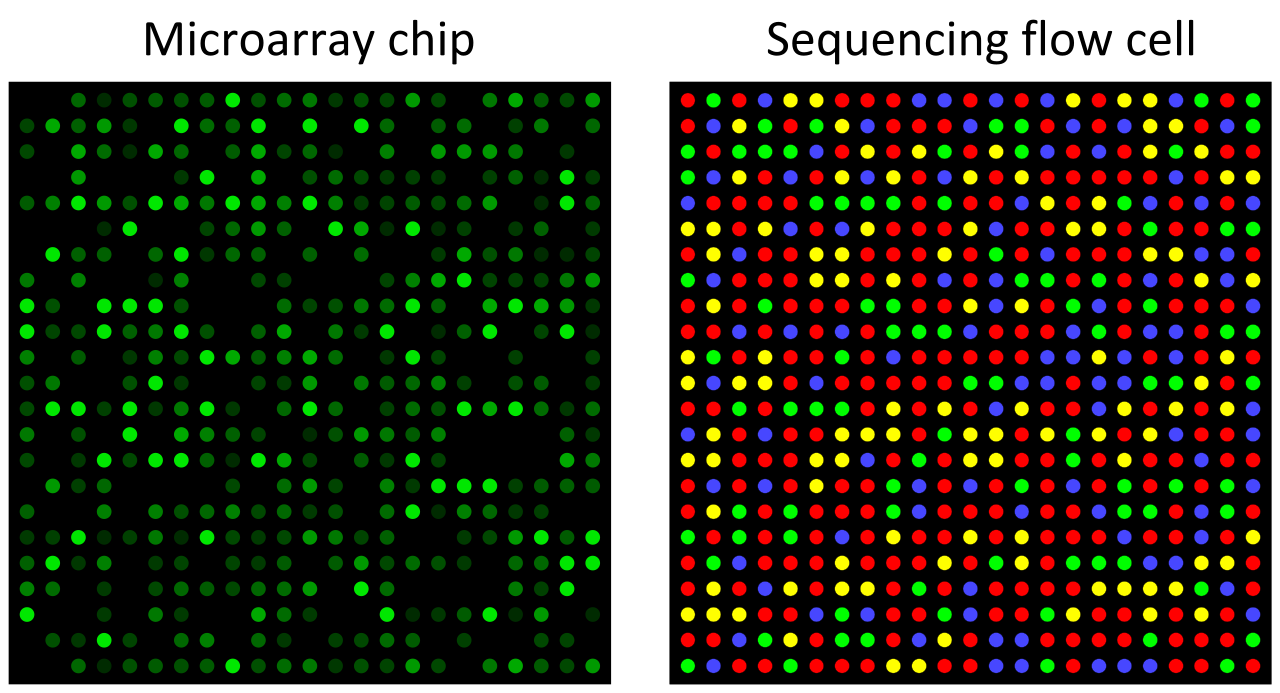
\includegraphics[scale = 0.25]{pictures/flow_cell.png}
	\caption{A single read or an illumni flow cell. This will be repeated for the entire length of the fragment.}
\end{figure}
This method introduces a few different QC issues. Namely for different length segments, we will see low diversity in certain regions of the grid. Issues surrounding this sequencing tool has been well studied and solutions to these problems exist and won't be discussed here. 

Once we have sequenced each fragment, the fragments need to be realigned to the genome. This alignment is the focus of many bioinformatists. TopHat and STAR offer computational solutions of fuzzy matching fragments to a reference genome. From here, we can attribute each read to each gene and begin constructing the reads per gene matrix. 

\subsection{Analysis}
Once we have arrived at our final read per gene matrix, a few normalization measures need to be taken. In particular the reads depend on the total library size as well as the gene length. For this reason we define the following normalized quantities. 
\begin{align*}
RPKM &= \frac{\#\text{Reads}}{\text{gene length}/1000 * \text{total no. reads}/1,000,000}\\
CPM &= \frac{\text{Reads Mapped to Gene}}{\text{total no. reads}*1,000,000}\\
FPKM &= \text{fragments per kilo base per million mapped fragments}
\end{align*}
FPKM is used for paired end reads. While these transformations are rather naive in practice, we can also develop count models such as Poission or Negative Binomial models. These two models are popularized by the software packages edgeR and DESeq2. 

\subsection{edgeR}
Suppose we have $n$ RNA-Seq sample that is sequenced, mapped to the genome, and the reads are counted by each gene. The number of reads for sample $i$ mapped to gene $g$ is given by $y_{gi}$. The set of genewise counts for sample $i$ makes up the \textit{library} for that sample. We then model the expected size of each count as the relative abundance times the library size ($m_i$). In this model, we model the entries of the reads per count matrix as a negative binomial. In particular, if we take the model 
\begin{align*}
	y_{gi}&\sim NB(m_i\lambda, \phi)\\
	f(y;\mu\phi) &= \frac{\Gamma(y+\phi^{-1})}{\Gamma(\phi^{-1})\Gamma(y+1)}\left(\frac{1}{1+\mu\phi}\right)^{\phi^{-1}}\left(\frac{\mu}{\phi^{-1}+\mu}\right)^{y}\\
	\E(Y) &= \mu, \V(Y) = \mu + \phi\mu^2
\end{align*}
If we suppose that the library size for each sample is equal across samples, we have 
\begin{align*}
	Z_g\equiv \sum_{i=1}^ny_{gi}&\sim NB(mn\lambda, \phi)
\end{align*}
From here we could just use conditional maximum likelihood conditioned on the number of reads for individual $i$
\begin{equation}
	\ell_{y_{gi}|Z = z}(\phi) = \sum_{i=1}^n\log\Gamma(y_{gi}+\phi^{-1}) + \log\Gamma(n\phi^{-1})-\log\Gamma(z+n\phi^{-1})-n\log\Gamma(\phi^{-1})
\end{equation}
In unequal library settings, we simply interpolate these counts as if they were from $NB(m^{*}\lambda, \phi)$ for $m^{*} =\left(\prod_{i=1}^nm_i\right)^{1/n}$. This interpolation follows the following procedure. 
\begin{enumerate}
	\item Initialize $\phi$
	\item Estimate $\lambda$ given $\phi$
	\item Find the proportion of $p_i$ of $y_i$ as follows $p_i = \prob(Y\leq y_i; m_i\lambda, \phi)+\frac{1}{2}\prob(Y=y_i; m_i\lambda, \phi)$ 
	\item Find the $p_{i}$th percentile assuming $NB(m^{*}\lambda, \phi)$. We call this the psuedo-data.
	\item Calculate $\phi$ using CML on the psuedo data
	\item Repeat until $\phi$ converges
\end{enumerate}
Another method that does not rely on assuming this equal library size is based on weighted likelihood function. 
\begin{equation}
	WL(\phi_{g}) = \mathcal{L}_g(\phi_g) + \alpha\mathcal{L}_c(\phi_g)
\end{equation}
Here the problem reduces to estimating $\alpha$. It does so by matching moments and normal approximations. 
\subsection{DESeq2}
A similar model to edgeR, DESeq2 uses a negative binomial model given by the following 
\begin{align*}
	y_{ij}&\sim NB(\mu_{ij}, \alpha_i)\\
	\mu_{ij}& = s_iq_{ij}\\
	s_i &= \text{median}_{y_i^R\neq 0}\frac{y_{ij}}{y_i^R}\quad y_i^r = \left(\prod_{j=1}^my_{ij}\right)^{1/m}\\
	\log q_{ij} &= \beta^Tx_j
\end{align*}
From here we estimate the dispersions using the Bayesian model 
\begin{align*}
	\log\alpha_i&\sim N(\log\alpha_{tr}(\overline{\mu}_i),\sigma_d^2)\\
	\overline{\mu}_i &= \frac{1}{m}\frac{Y_{ij}}{s_j}
\end{align*}
For details see the lecture slides. In essence this is an extension of edgeR to a Bayesian framework. 

\subsection{Voom + limma}
Perhaps the most simple model, we just use a linear model with $\log(CPM)$ where we precision is adjusted by using the weights of the mean-variance relation. 


\end{document}








































